\documentclass[a4paper,11pt]{article}
\usepackage[a4paper]{geometry}
\usepackage[utf8]{inputenc}

\title{Advanced Solid State Physics Course Notes \\ DTU Course 10305}
\author{Lecturer: \emph{Kristian Thygesen}}
\date{Fall 2018}

%%%%%%%%%%%%%%%%%%%%%%%%%%%%%%%%%%%%%%%%%%
%            Packages                    %
%%%%%%%%%%%%%%%%%%%%%%%%%%%%%%%%%%%%%%%%%%
\usepackage{amsfonts,amsmath,amssymb} % Math symbols form American Mathematical Society
\usepackage[english]{babel} 
\usepackage{textcomp}
\usepackage{bm}
\usepackage{makeidx}
\usepackage{graphicx}
\usepackage{amsthm}
\usepackage{enumerate}% http://ctan.org/pkg/enumerate


%%%%%%%%%%%%%%%%%%%%%%%%%%%%%%%%%%%%%%%%%%
%               Newcommands              %
%%%%%%%%%%%%%%%%%%%%%%%%%%%%%%%%%%%%%%%%%%

% BATMAN
\newcommand{\batmanPic}[1]{
    \begin{tikzpicture}[baseline=0em, scale=#1]
        \draw[fill,black]   (-0.25,1.48) .. controls (-0.1,1.5) and (0.1,1.5) .. (0.25,1.48) -- (0.35,1.92) .. controls (0.425,1.8) and (0.41,1.3) .. (0.45,1.2) .. controls (0.6,1.05) and (1.96,1.05) .. (1.98,2.08) -- (5.93,2.08) .. controls (4.2,1.45) and (4,0.3) .. (4.2,-0.28) .. controls (2.4,-0.09) and (0.4,-0.5) .. (0,-2.052) .. controls (-0.4,-0.5) and (-2.4,-0.09) .. (-4.2,-0.28) .. controls (-4,0.3) and (-4.2,1.45) .. (-5.93,2.08) -- (-1.98,2.08) .. controls (-1.96,1.05) and (-0.6,1.05) .. (-0.45,1.2) .. controls (-0.41,1.3) and (-0.425,1.8) .. (-0.35,1.92) -- (-0.25,1.48);
    \end{tikzpicture}
    
} % End of \batman command
\newcommand{\batman}{\batmanPic{0.05}}
\renewcommand\qedsymbol{\batman}

% SMART COMMANDS FOR THIS PROJECT
\DeclareMathOperator*{\argmin}{\arg\!\min}
\DeclareMathOperator*{\argmax}{\arg\!\max}
\newcommand{\Lnorm}[1]{$L_{#1}$-norm}
\newcommand{\R}{\mathbb{R}}
\newcommand{\C}{\mathbb{C}}
\newcommand{\bsw}{\boldsymbol{w}}
\newcommand{\cov}{\mathrm{c\hat{o}v}}
\newcommand{\covm}{\boldsymbol{\Sigma}}
\newcommand{\curlyb}[1]{\left\{ {#1} \right\}}
\newcommand{\Egeneral}{E_{\mathcal{M}}^{\mathrm{gen}}}
\newcommand{\Dtrain}{\mathcal{D}_{\mathrm{train}}}
\newcommand{\Dtest}{\mathcal{D}_{\mathrm{test}}}
\newcommand{\EM}[1]{\hat{E}_{\mathcal{M}}^{\mathrm{#1}}}
\newcommand{\EMss}[2]{E_{{\mathcal{M}#1}}^{{\mathrm{#2}}}}
\newcommand{\FM}[1]{f_{\mathcal{M}}\qty(#1)}
\newcommand{\calDss}[2]{\mathcal{D}_{{#1}}^{{\mathrm{#2}}}}
\newcommand{\RMSE}{\mathrm{RMSE}}
\newcommand{\hadd}{h_{add}}
\newcommand{\hast}{h^{\ast}}
\newcommand{\fop}[1]{\boldsymbol{\Psi}\qty(#1)}
\newcommand{\fopd}[1]{\boldsymbol{\Psi}^{\dagger}\qty(#1)}
\newcommand{\expe}[1]{\mathrm{e}^{{#1}}}
% NEW THEOREM ENVIRONMENT: Exercise
\newtheorem{exercise}{Exercise}
\newtheorem{solution}{Solution}


% SPACINGS
\newcommand{\linie}{\underline{\makebox[\textwidth]{}}}
\newcommand{\spacer}{\rule[-2mm]{0mm}{6mm}}
\newcommand{\notop}{{{}_{}}}
\newcommand{\ontop}[1]{{{#1}_{}}}
%
% LITERAL ABBREVIATIONS
\newcommand{\ie}{i.e.}
\newcommand{\eg}{e.g.}
\newcommand{\etc}{\textit{etc.}}
\newcommand{\etal}{\textit{et~al.}}
\newcommand{\MICDTU}{DTU Nanotech}
%
% MATH SYMBOLS

\renewcommand{\vec}[1]{\bm{#1}}
\newcommand{\vb}[1]{\bm{#1}}
\newcommand{\difd}{\mathrm{d}}
\newcommand{\ee}{\mathrm{e}}
\newcommand{\ii}{\mathrm{i}}
\newcommand{\dm}{\mathrm{d}}
\newcommand{\sgn}{\mathrm{sgn}}
\newcommand{\sm}{\!-\!}
\newcommand{\sP}{\!+\!}
\newcommand{\im}{\mathrm{Im}}
\newcommand{\re}{\mathrm{Re}}
\newcommand{\krondel}[2]{\delta^\notop_{#1 #2}}
\newcommand{\Tr}{\mathrm{Tr}}
\newcommand{\ion}{\ii\omega^\notop_n}
\newcommand{\iot}{\ii\omega t}
\newcommand{\taun}{\tau^\notop}
\newcommand{\lam}{\lambda}
\newcommand{\lamn}{\lambda^{{}}}
\newcommand{\limit}[2]{\mathop{\longrightarrow}_{#1 \rightarrow #2}}
\newcommand{\gamn}{\gamma^{{}}}
\newcommand{\nun}{\nu^\notop}
\newcommand{\ve}{\varepsilon}
\newcommand{\ven}{\ve^\notop}
\newcommand{\xin}{\xi^\notop}
\newcommand{\zetan}{\zeta^\notop}
\newcommand{\pp}{\partial^{{}}}
\newcommand{\ppsqr}{\partial^{\,2_{}}}
\newcommand{\nablabf}{\boldsymbol{\nabla}}
\newcommand{\nablabfn}{\boldsymbol{\nabla}^\notop}
\newcommand{\Lapl}{\nabla^2}
\newcommand{\nablasqr}{\nabla^2}
\newcommand{\rot}{\nablabf\times}
\newcommand{\divop}{\nablabf\scap}
%
% MATH STYLE
\newcommand{\scap}{\!\cdot\!}
\newcommand{\intd}[1]{{\int\!\dm#1\: }}
\newcommand{\inttau}[1]{{\int_0^\beta\!d\tauno_{#1}\: }}
\newcommand{\dpst}{\displaystyle}
\newcommand{\scst}{\scriptstyle}
\newcommand{\scscst}{\scriptscriptstyle}
\newcommand{\fracsmall}[2]{\mbox{$\frac{#1}{#2}$}}
\newcommand{\sqrtsmall}[1]{\mbox{$\sqrt{#1}$}}
\newcommand{\half}{\fracsmall{1}{2}}
\newcommand{\third}{\fracsmall{1}{3}}
\newcommand{\quarter}{\fracsmall{1}{4}}
%
% BOLD SYMBOLS
\newcommand{\AAA}{\vec{A}}
\newcommand{\AAn}{\vec{A}^\notop}
\newcommand{\Ann}{A^\notop}
\newcommand{\aaa}{\vec{a}}
\newcommand{\aan}{\vec{a}^\notop}
\newcommand{\ann}{a^\notop}
\newcommand{\asqr}{a^{2_{}}}
\newcommand{\BBB}{\vec{B}}
\newcommand{\BBn}{\vec{B}^\notop}
\newcommand{\Bnn}{B^\notop}
\newcommand{\bbb}{\vec{b}}
\newcommand{\bbn}{\vec{b}^\notop}
\newcommand{\bnn}{b^\notop}
\newcommand{\bsqr}{b^{2_{}}}
\newcommand{\CCC}{\vec{C}}
\newcommand{\CCn}{\vec{C}^\notop}
\newcommand{\CD}{C^\notop_\mathrm{D}}
\newcommand{\Cs}{C^\notop_\mathrm{s}}
\newcommand{\ccc}{\vec{c}}
\newcommand{\ccn}{\vec{c}^\notop}
\newcommand{\cnn}{c^\notop}
\newcommand{\DDD}{\vec{D}}
\newcommand{\DDn}{\vec{D^\notop}}
\newcommand{\ddd}{\vec{d}}
\newcommand{\ddn}{\vec{d^\notop}}
\newcommand{\EEE}{\vec{E}}
\newcommand{\EEn}{\vec{E^\notop}}
\newcommand{\Enn}{E^\notop}
\newcommand{\eee}{\vec{e}}
\newcommand{\een}{\vec{e}^\notop}
\newcommand{\FFF}{\vec{F}}
\newcommand{\FFn}{\vec{F}^\notop}
\newcommand{\Fnn}{F^\notop}
\newcommand{\FFFe}{\vec{F}^\notop_\mathrm{el}}
\newcommand{\fff}{\vec{f}}
\newcommand{\ffn}{\vec{f}^\notop}
\newcommand{\fnn}{f^\notop}
\newcommand{\fffe}{\vec{f}^\notop_\mathrm{el}}
\newcommand{\GGn}{\vec{G}}
\newcommand{\GGG}{\vec{G}^\notop}
\newcommand{\ggn}{\vec{g}^\notop}
\newcommand{\gnn}{g^\notop}
\newcommand{\HHH}{\vec{H}}
\newcommand{\HHn}{\vec{H}^\notop}
\newcommand{\iii}{\vec{i}}
\newcommand{\iin}{\vec{i}^\notop}
\newcommand{\JJJ}{\vec{J}}
\newcommand{\JJn}{\vec{J}^\notop}
\newcommand{\Jnn}{J^\notop}
\newcommand{\JJJe}{\vec{J}^\notop_\mathrm{el}}
\newcommand{\JJJti}{\vec{\tilde{J}}}
\newcommand{\JJnti}{\vec{\tilde{J}}^\notop}
\newcommand{\JJdiff}{\vec{J}^{\mathrm{diff}_{}}}
\newcommand{\Jdiff}{J^{\mathrm{diff}_{}}}
\newcommand{\JJext}{\vec{J}^{{}}_{\mathrm{ext}}}
\newcommand{\JJmag}{\vec{J}^{{}}_{\mathrm{mag}}}
\newcommand{\JJheat}{\vec{J}^{{}}_{\mathrm{heat}}}
\newcommand{\Jheat}{J^{{}}_{\:\mathrm{heat}}}
\newcommand{\JJhcond}{\vec{J}^\mathrm{cond}_\mathrm{heat}}
\newcommand{\Jhcond}{J^{\:\mathrm{cond}}_{\:\:\mathrm{heat}}}
\newcommand{\JJhconv}{\vec{J}^\mathrm{conv}_\mathrm{heat}}
\newcommand{\Jhconv}{J^{\:\mathrm{conv}}_{\:\:\mathrm{heat}}}
\newcommand{\kkk}{\vec{k}}
\newcommand{\kkn}{\vec{k}^\notop}
\newcommand{\knn}{k^\notop}
\newcommand{\ksqr}{k^{2_{}}}
\newcommand{\KKK}{\vec{K}}
\newcommand{\KKn}{\vec{K}^\notop}
\newcommand{\MMM}{\vec{M}}
\newcommand{\MMn}{\vec{M}^\notop}
\newcommand{\mmm}{\vec{m}}
\newcommand{\mmn}{\vec{m}^\notop}
\newcommand{\nnn}{\vec{n}}
\newcommand{\nnnn}{\vec{n}^\notop}
\newcommand{\PPP}{\vec{P}}
\newcommand{\PPn}{\vec{P}^\notop}
\newcommand{\ppp}{\vec{p}}
\newcommand{\ppn}{\vec{p}^\notop}
\newcommand{\pnn}{p^\notop}
\newcommand{\QQQ}{\vec{Q}}
\newcommand{\QQn}{\vec{Q}^\notop}
\newcommand{\Qnn}{Q^\notop}
\newcommand{\qqq}{\vec{q}}
\newcommand{\qqn}{\qqq^\notop}
\newcommand{\RRR}{\vec{R}}
\newcommand{\RRn}{\RRR^\notop}
\newcommand{\Rnn}{R^\notop}
\newcommand{\rrr}{\vec{r}}
\newcommand{\rrn}{\rrr^\notop}
\newcommand{\rij}{r^\notop_{ij}}
\newcommand{\sss}{\vec{s}}
\newcommand{\ssn}{\sss^\notop}
\newcommand{\snn}{s^\notop}
\newcommand{\ssqr}{s^{2_{}}}
\newcommand{\Tnn}{{T}^\notop}
\newcommand{\uuu}{\vec{u}}
\newcommand{\uun}{\vec{u}^\notop}
\newcommand{\unn}{{u}^\notop}
\newcommand{\VVV}{\vec{V}}
\newcommand{\VVn}{\vec{V}^\notop}
\newcommand{\Vnn}{{V}^\notop}
\newcommand{\VLJ}{{V}^\notop_\mathrm{LJ}}
\newcommand{\vvv}{\vec{v}}
\newcommand{\vvn}{\vec{v}^\notop}
\newcommand{\vnn}{{v}^\notop}
\newcommand{\www}{\vec{w}}
\newcommand{\wwn}{\vec{w}^\notop}
\newcommand{\wnn}{{w}^\notop}
\newcommand{\wdd}{w^{{}}_\mathrm{d}}
\newcommand{\xxx}{\vec{x}}
\newcommand{\xxn}{\xxx^\notop}
\newcommand{\XXX}{\vec{X}}
\newcommand{\xnn}{x^\notop}
\newcommand{\yyy}{\vec{y}}
\newcommand{\Znn}{Z^\notop}
\newcommand{\znn}{z^\notop}
\newcommand{\zerovec}{\boldsymbol{0}}
%
% PHYSICS SYMBOLS
\newcommand{\calA}{\mathcal{A}}
\newcommand{\calC}{\mathcal{C}}
\newcommand{\calCn}{\mathcal{C}^{{}}}
\newcommand{\calD}{\mathcal{D}}
\newcommand{\calDn}{\mathcal{D}^{{}}}
\newcommand{\calO}{\mathcal{O}}
\newcommand{\calP}{\mathcal{P}}
\newcommand{\calPO}{\mathcal{P}^{{}}_0}
\newcommand{\calPs}{\mathcal{P}^{{}}_\mathrm{s}}
\newcommand{\calPf}{\mathcal{P}^{{}}_\mathrm{f}}
\newcommand{\calR}{\mathcal{R}}
\newcommand{\calT}{\mathcal{T}}
\newcommand{\calV}{\mathcal{V}}
\newcommand{\area}{\mathcal{A}}
\newcommand{\aI}{{a^{{}}_1}}
\newcommand{\aIsqr}{{a^{2_{}}_1}}
\newcommand{\aIcub}{{a^{3_{}}_1}}
\newcommand{\aII}{{a^{{}}_2}}
\newcommand{\aIIsqr}{{a^{2_{}}_2}}
\newcommand{\aIIcub}{{a^{3_{}}_2}}
\newcommand{\aB}{{a^\notop_0}}
\newcommand{\ath}{{a^\notop_\mathrm{th}}}
\newcommand{\ap}{{a^\notop_\mathrm{p}}}
\newcommand{\aexp}{{a^\notop_\mathrm{exp}}}
\newcommand{\alphap}{\alpha^{{}}_\mathrm{p}}
\newcommand{\aeta}{{\alpha^\notop_\eta}}
\newcommand{\akap}{{\alpha^\notop_\kappa}}
\newcommand{\arho}{{\alpha^\notop_\rho}}
\newcommand{\aetasqr}{{\alpha^{2_{}}_\eta}}
\newcommand{\akapsqr}{{\alpha^{2_{}}_\kappa}}
\newcommand{\arhosqr}{{\alpha^{2_{}}_\rho}}
\newcommand{\BO}{\textit{Bo}}
\newcommand{\CCD}{C^{{}}_\mathrm{D}}
\newcommand{\Chyd}{C^{{}}_\mathrm{hyd}}
\newcommand{\CA}{\textit{Ca}}
\newcommand{\CCa}{C^{{}}_\alpha}
\newcommand{\cca}{c^{{}}_\alpha}
\newcommand{\ca}{c^{{}}_\mathrm{a}}
\newcommand{\casqr}{c^{2_{}}_\mathrm{a}}
\newcommand{\cm}{c^{{}}_\mathrm{m}}
\newcommand{\cmO}{c^{(0)_{}}_\mathrm{m}}
\newcommand{\cmI}{c^{(1)_{}}_\mathrm{m}}
\newcommand{\cmII}{c^{(2)_{}}_\mathrm{m}}
\newcommand{\cmi}{c^{(i)_{}}_\mathrm{m}}
\newcommand{\co}{c^{{}}_\mathrm{o}}
\newcommand{\cp}{c^{{}}_\mathrm{p}}
\newcommand{\cpm}{c^{{}}_\pm}
\newcommand{\cpp}{c^{{}}_+}
\newcommand{\cmm}{c^{{}}_-}
\newcommand{\Cth}{C^\notop_\mathrm{th}}
\newcommand{\dktwopicubed}{\frac{d\kkk}{\twopicubed}}
\newcommand{\Deln}{\Delta^\notop}
\newcommand{\Dth}{D^\notop_\mathrm{th}}
\newcommand{\Ekin}{E^{{}}_\mathrm{kin}}
\newcommand{\Etot}{E_\mathrm{tot}}
\newcommand{\ffe}{\fff^{{}}_\mathrm{el}}
\newcommand{\FC}{\mathcal{F}}
\newcommand{\FFFdip}{\FFF^{{}}_\mathrm{dip}}
\newcommand{\FFFDEP}{\FFF^{{}}_\mathrm{DEP}}
\newcommand{\FFFdrag}{\FFF^{{}}_\mathrm{drag}}
\newcommand{\Fimp}{F^{{}}_\mathrm{imp}}
\newcommand{\GC}{G}
\newcommand{\GCn}{G^{{}}}
\newcommand{\Ghyd}{G^{{}}_\mathrm{hyd}}
\newcommand{\hc}{h^{{}}_\mathrm{c}}
\newcommand{\hf}{h^{{}}_\mathrm{f}}
\newcommand{\Dh}{\Delta h}
\newcommand{\IO}{I^{{}}_0}
\newcommand{\Is}{I^{{}}_\mathrm{s}}
\newcommand{\If}{I^{{}}_\mathrm{f}}
\newcommand{\Ith}{I^\notop_\mathrm{th}}
\newcommand{\Ieo}{I^\notop_\mathrm{eo}}
\newcommand{\Ieocond}{I^{\textrm{cond}_{}}_\mathrm{eo}}
\newcommand{\Ieoconv}{I^{\textrm{conv}_{}}_\mathrm{eo}}
\newcommand{\Ipconv}{I^{\textrm{conv}_{}}_\mathrm{p}}
\newcommand{\kB}{{k^\notop_\mathrm{B}}}
\newcommand{\kBT}{{k^\notop_\mathrm{B} T}}
\newcommand{\Lc}{L^{{}}_\mathrm{c}}
\newcommand{\Lx}{L^{{}}_x}
\newcommand{\Ly}{L^{{}}_y}
\newcommand{\Lz}{L^{{}}_z}
\newcommand{\elln}{\ell^\notop}
\newcommand{\elli}{{\ell^{{}}_\mathrm{i}}}
\newcommand{\ello}{{\ell^{{}}_\mathrm{o}}}
\newcommand{\elld}{{\ell^{{}}_\mathrm{d}}}
\newcommand{\ellc}{\ell^{{}}_\mathrm{c}}
\newcommand{\lcap}{\ell^{{}}_\mathrm{cap}}
\newcommand{\lcapsqr}{\ell^{2_{}}_\mathrm{cap}}
\newcommand{\len}{\mathcal{L}}
\newcommand{\nre}{n^{{}}_\mathrm{re}}
\newcommand{\nim}{n^{{}}_\mathrm{im}}
\newcommand{\nnp}{n^{+_{}}}
\newcommand{\nnm}{n^{-_{}}}
\newcommand{\npm}{n^{\pm_{}}}
\newcommand{\nin}{n^\notop_\mathrm{in}}
\newcommand{\nout}{n^\notop_\mathrm{out}}
\newcommand{\Ps}{P^{{}}_\mathrm{s}}
\newcommand{\pc}{{p^{{}}_\mathrm{c}}}
\newcommand{\peo}{p^\notop_\mathrm{eo}}
\newcommand{\phs}{p^{{}}_\mathrm{hs}}
\newcommand{\ptot}{p^{{}}_\mathrm{tot}}
\newcommand{\pimp}{p^{{}}_\mathrm{imp}}
\newcommand{\pL}{{p^{{}}_\mathrm{L}}}
\newcommand{\pR}{{p^{{}}_\mathrm{R}}}
\newcommand{\pii}{{p^{{}}_{\,\mathrm{i}}}}
\newcommand{\piiI}{{p^{{}}_{\,\mathrm{i},1}}}
\newcommand{\piiII}{{p^{{}}_{\,\mathrm{i},2}}}
\newcommand{\poo}{{p^{{}}_\mathrm{o}}}
\newcommand{\pdd}{{p^{{}}_\mathrm{d}}}
\newcommand{\pww}{{p^{{}}_\mathrm{w}}}
\newcommand{\Dp}{\Delta p}
\newcommand{\Dpn}{\Delta p^{{}}}
\newcommand{\dpb}{\Delta p^{{}}_\mathrm{b}}
\newcommand{\Dpb}{\Delta p^{{}}_\mathrm{b}}
\newcommand{\pclog}{p^{{}}_\mathrm{clog}}
\newcommand{\Dpsurf}{\Delta p^{{}}_\mathrm{surf}}
\newcommand{\DPsurf}{\Delta p^{{}}_\mathrm{surf}}
\newcommand{\DP}{\Delta P}
\newcommand{\Peth}{\PE^{{}}_\mathrm{th}}
\newcommand{\PE}{\textit{P\'e}}
\newcommand{\Qc}{Q^{{}}_\mathrm{c}}
\newcommand{\Qcav}{Q^\notop_\mathrm{c}}
\newcommand{\Qeo}{Q^\notop_\mathrm{eo}}
\newcommand{\QeoS}{Q^{*_{}}_\mathrm{eo}}
\newcommand{\Qexp}{Q^\notop_\mathrm{exp}}
\newcommand{\Qmass}{Q^\notop_\mathrm{mass}}
\newcommand{\QmassO}{Q^\notop_{\textrm{mass},0}}
\newcommand{\Qtot}{Q^\notop_\mathrm{tot}}
\newcommand{\Qp}{Q^\notop_\mathrm{p}}
\newcommand{\Qii}{{Q^{{}}_\mathrm{i}}}
\newcommand{\Qoo}{{Q^{{}}_\mathrm{o}}}
\newcommand{\Qdd}{{Q^{{}}_\mathrm{d}}}
\newcommand{\Qth}{Q^\notop_\mathrm{th}}
\newcommand{\QthS}{Q^{*_{}}_\mathrm{th}}
\newcommand{\RE}{\textit{Re}}
\newcommand{\RcI}{R^{\mathrm{c}_{}}_1}
\newcommand{\RcII}{R^{\mathrm{c}_{}}_2}
\newcommand{\Rh}{R^{{}}_\mathrm{hyd}}
\newcommand{\RhS}{R^{*_{}}_\mathrm{hyd}}
\newcommand{\Rhyd}{R^{{}}_\mathrm{hyd}}
\newcommand{\RhydS}{R^{*_{}}_\mathrm{hyd}}
\newcommand{\Rhydp}{R^{\textrm{p}_{}}_\mathrm{hyd}}
\newcommand{\Rhydexp}{R^{\textrm{exp}_{}}_\mathrm{hyd}}
\newcommand{\Rth}{R^\notop_\mathrm{th}}
\newcommand{\DS}{\Delta S}
\newcommand{\Tg}{T^{{}}_\mathrm{g}}
\newcommand{\Tc}{T^{{}}_\mathrm{c}}
\newcommand{\Dt}{\Delta t}
\newcommand{\DT}{\Delta T}
\newcommand{\tacc}{\tau^{{}}_\mathrm{acc}}
\newcommand{\tadv}{\tau^{{}}_\mathrm{adv}}
\newcommand{\tcap}{\tau^{{}}_\mathrm{cap}}
\newcommand{\timp}{\tau^{{}}_\mathrm{imp}}
\newcommand{\tdiff}{\tau^{{}}_\mathrm{diff}}
\newcommand{\tdiffa}{\tau^{\textrm{ax}_{}}_\mathrm{diff}}
\newcommand{\tdiffr}{\tau^{\textrm{rad}_{}}_\mathrm{diff}}
\newcommand{\tconv}{\tau^{{}}_\mathrm{conv}}
\newcommand{\tconva}{\tau^{{L^{{}}_{}}}_\mathrm{conv}}
\newcommand{\tconvr}{\tau^{{a^{{}}_{}}}_\mathrm{conv}}
\newcommand{\tRC}{\tau^{{}}_{RC}}
\newcommand{\vol}{\mathcal{V}}
\newcommand{\vg}{\vnn_\mathrm{g}}
\newcommand{\veo}{\vnn_\mathrm{eo}}
\newcommand{\vvvwall}{\vvn_\mathrm{wall}}
\newcommand{\DV}{\Delta V}
\newcommand{\xc}{{x^{{}}_\mathrm{c}}}
\newcommand{\xcm}{{x^{{}}_\mathrm{cm}}}
\newcommand{\xL}{{x^{{}}_\mathrm{L}}}
\newcommand{\xR}{{x^{{}}_\mathrm{R}}}
\newcommand{\Dx}{\Delta x}
\newcommand{\Dy}{\Delta y}
\newcommand{\Dz}{\Delta z}
\newcommand{\zc}{{z^{{}}_\mathrm{c}}}
\newcommand{\deltan}{\delta^\notop}
\newcommand{\eps}{\epsilon}
\newcommand{\epsn}{\epsilon^{{}}}
\newcommand{\epss}{\epsilon^\notop_\mathrm{s}}
\newcommand{\epsO}{\epsilon^\notop_0}
\newcommand{\epsI}{\epsilon^\notop_1}
\newcommand{\epsII}{\epsilon^\notop_2}
\newcommand{\epsr}{\epsilon^\notop_\mathrm{r}}
\newcommand{\etan}{\eta^{{}}}
\newcommand{\etaeff}{\eta^{{}}_\mathrm{eff}}
\newcommand{\etaO}{\eta^{{}}_0}
\newcommand{\etap}{\eta^{\prime_{}}_0}
\newcommand{\etaS}{\eta^*}
\newcommand{\gamD}{\dot{\gamma}}
\newcommand{\gamDn}{\dot{\gamma}^{{}}}
\newcommand{\gamS}{\gamma^{*_{}}}
\newcommand{\gsl}{\gamma_\mathrm{sl}}
\newcommand{\gsg}{\gamma_\mathrm{sg}}
\newcommand{\glg}{\gamma_\mathrm{lg}}
\newcommand{\bfGamma}{\mbox{$\Gamma$\hspace*{-0.6em}$\Gamma$}}
\newcommand{\lamO}{\lambda^{{}}_0}
\newcommand{\lamnn}{\lambda^{{}}_n}
\newcommand{\lamnN}{\lambda^{(N)_{}}_n}
\newcommand{\lamD}{\lambda^{{}}_\mathrm{D}}
\newcommand{\lamDsqr}{\lambda^{{2}}_\mathrm{D}}
\newcommand{\lams}{\lambda^{{}}_\mathrm{s}}
\newcommand{\lamp}{\lambda^{{}}_+}
\newcommand{\lamppp}{\lambda^{\prime\prime_{}}_+}
\newcommand{\lampsqr}{\lambda^{2_{}}_+}
\newcommand{\lampcub}{\lambda^{3_{}}_+}
\newcommand{\lamm}{\lambda^{{}}_-}
\newcommand{\lammpp}{\lambda^{\prime\prime_{}}_-}
\newcommand{\lammsqr}{\lambda^{2_{}}_-}
\newcommand{\lammcub}{\lambda^{3_{}}_-}
\newcommand{\muO}{\mu^{{}}_0}
\newcommand{\mur}{\mu^\notop_\mathrm{r}}
\newcommand{\muion}{\mu^\notop_\mathrm{ion}}
\newcommand{\mueo}{\mu^\notop_\mathrm{eo}}
\newcommand{\oc}{{\omega^\notop_\mathrm{c}}}
\newcommand{\on}{{\omega^\notop_n}}
\newcommand{\ocsqr}{{\omega^{2_{}}_\mathrm{c}}}
\newcommand{\oD}{{\omega^\notop_\mathrm{D}}}
\newcommand{\phin}{\phi^{{}}}
\newcommand{\phiS}{\phi^{*_{}}}
\newcommand{\twopicubed}{(2\pi)^3}
\newcommand{\rhoe}{\rho^\notop_\mathrm{el}}
\newcommand{\rhon}{\rho^\notop}
\newcommand{\sigmae}{\sigma^\notop_\mathrm{el}}
\newcommand{\sigmaI}{\sigma^\notop_\mathrm{el,1}}
\newcommand{\sigmaII}{\sigma^\notop_\mathrm{el,2}}
\newcommand{\sigmaion}{\sigma^\notop_\mathrm{ion}}
\newcommand{\sigmaionp}{\sigma^{+_{}}_\mathrm{ion}}
\newcommand{\sigmaionm}{\sigma^{-_{}}_\mathrm{ion}}
\newcommand{\sigmaionpm}{\sigma^{\pm_{}}_\mathrm{ion}}
\newcommand{\sigman}{\sigma^\notop}
\newcommand{\domegatwopi}{\frac{d\omega}{2\pi}}
%
% Symbols with a tilde
\newcommand{\ctin}{{\tilde{c}^{{}}_n{}}}
\newcommand{\hti}{\tilde{h}}
\newcommand{\Lti}{{\tilde{L}^{{}}{}}}
\newcommand{\pti}{{\tilde{p}^{{}}{}}}
\newcommand{\ptiO}{\tilde{p}^{(0)_{}}}
\newcommand{\ptiI}{\tilde{p}^{(1)_{}}}
\newcommand{\ppti}{{\tilde{\partial}^{{}}{}}}
\newcommand{\rti}{{\tilde{r}^{{}}{}}}
\newcommand{\rrrti}{{\tilde{\rrr}^{{}}{}}}
\newcommand{\tti}{{\tilde{t}^{{}}{}}}
\newcommand{\ttiO}{\tilde{t}^{{}}_0}
\newcommand{\uti}{{\tilde{u}^{{}}{}}}
\newcommand{\utin}{{\tilde{u}^{{}}_n{}}}
\newcommand{\utim}{{\tilde{u}^{{}}_m{}}}
\newcommand{\vti}{{\tilde{v}^{{}}{}}}
\newcommand{\vtiO}{\tilde{v}^{(0)_{}}}
\newcommand{\vtiI}{\tilde{v}^{(1)_{}}}
\newcommand{\vxti}{{\tilde{v}^{{}}_x{}}}
\newcommand{\vvvti}{{\tilde{\vvv}^{{}}{}}}
\newcommand{\xti}{{\tilde{x}^{{}}{}}}
\newcommand{\xtiO}{\tilde{x}^{{}}_0}
\newcommand{\xtiI}{\tilde{x}^{{}}_1}
\newcommand{\yti}{{\tilde{y}^{{}}{}}}
\newcommand{\zti}{{\tilde{z}^{{}}{}}}
\newcommand{\phiti}{{\tilde{\phi}^{{}}{}}}
\newcommand{\nablati}{{\tilde{\nablabf}^{{}}{}}}
\newcommand{\XXXtilde}{\tilde{\vec{X}}}
%
% Symbols with a subscript 0, 1, or 2
\newcommand{\CO}{C^{{}}_0}
\newcommand{\cO}{c^{{}}_0}
\newcommand{\cOsqr}{c^{\:2_{}}_0}
\newcommand{\EO}{E^{{}}_0}
\newcommand{\EEEO}{\EEE^{{}}_0}
\newcommand{\FO}{F^{{}}_0}
\newcommand{\FFFII}{\FFF^{{}}_2}
\newcommand{\FFFIIav}{\langle\FFF^{{}}_2\rangle^{{}}_{t^{}}}
\newcommand{\hO}{h^{{}}_0}
\newcommand{\hOsqr}{h^{2_{}}_0}
\newcommand{\hOcub}{h^{3_{}}_0}
\newcommand{\HO}{H^{{}}_0}
\newcommand{\kO}{k^{{}}_0}
\newcommand{\kOsqr}{k^{_{}}_0}
\newcommand{\kn}{k^{{}}_n}
\newcommand{\kapn}{\kappa^{{}}}
\newcommand{\kapO}{\kappa^{{}}_0}
\newcommand{\kapI}{\kappa^{{}}_1}
\newcommand{\kapII}{\kappa^{{}}_2}
\newcommand{\LO}{L^{{}}_0}
\newcommand{\LOsqr}{L^{2_{}}_0}
\newcommand{\mmmII}{\mmm^{{}}_2}
\newcommand{\nO}{n^{{}}_0}
\newcommand{\NO}{N^{{}}_0}
\newcommand{\omegabf}{\boldsymbol{\omega}}
\newcommand{\oO}{{\omega^\notop_\mathrm{0}}}
\newcommand{\oOsqr}{{\omega^{2_{}}_\mathrm{0}}}
\newcommand{\ocN}{\omega^{(N)_{}}_\mathrm{c}}
\newcommand{\olaser}{\omega^{{}}_\mathrm{laser}}
\newcommand{\pO}{p^{{}}_0}
\newcommand{\pS}{p^*}
\newcommand{\pI}{p^{{}}_1}
\newcommand{\pII}{p^{{}}_2}
\newcommand{\PO}{P^{{}}_0}
\newcommand{\QO}{Q^{{}}_0}
\newcommand{\QI}{Q^{{}}_1}
\newcommand{\rO}{r^{{}}_0}
\newcommand{\rOsqr}{r^{2_{}}_0}
\newcommand{\RO}{R^\notop_0}
\newcommand{\RI}{R^\notop_1}
\newcommand{\RII}{R^\notop_2}
\newcommand{\RIII}{R^\notop_3}
\newcommand{\SO}{S^{{}}_0}
\newcommand{\so}{s^{{}}_\mathrm{o}}
\newcommand{\sosqr}{s^{2_{}}_\mathrm{o}}
\newcommand{\tO}{t^{{}}_0}
\newcommand{\tth}{t^{{}}_\mathrm{th}}
\newcommand{\tauO}{\tau^{{}}_0}
\newcommand{\tauI}{\tau^{{}}_1}
\newcommand{\tauth}{\tau^{{}}_\mathrm{th}}
\newcommand{\thetan}{\theta^{{}}}
\newcommand{\thetat}{\theta^{{}}_\mathrm{t}}
\newcommand{\thetaO}{\theta^{{}}_0}
\newcommand{\thetaI}{\theta^{{}}_1}
\newcommand{\ThetaO}{\Theta^{{}}_0}
\newcommand{\ThetaI}{\Theta^{{}}_1}
\newcommand{\TO}{T^{{}}_0}
\newcommand{\uO}{u^{{}}_0}
\newcommand{\VO}{V^{{}}_0}
\newcommand{\VOsqr}{V^{2_{}}_0}
\newcommand{\vO}{v^{{}}_0}
\newcommand{\vvvO}{\vvv^{{}}_0}
\newcommand{\VVVO}{\VVV^{{}}_0}
\newcommand{\vI}{v^{{}}_1}
\newcommand{\vvvI}{\vvv^{{}}_1}
\newcommand{\vII}{v^{{}}_2}
\newcommand{\vvvII}{\vvv^{{}}_2}
\newcommand{\uI}{u^{{}}_1}
\newcommand{\xO}{x^{{}}_0}
\newcommand{\xI}{x^{{}}_1}
\newcommand{\yO}{y^{{}}_0}
\newcommand{\zab}{z^{{}}_{ab}}
\newcommand{\zO}{z^{{}}_0}
\newcommand{\zOsqr}{z^{2_{}}_0}
\newcommand{\volS}{\vol^*}
\newcommand{\volO}{\vol^{{}}_0}
\newcommand{\phiO}{\phi^{{}}_0}
\newcommand{\phiI}{\phi^{{}}_1}
\newcommand{\phiII}{\phi^{{}}_2}
\newcommand{\rhoO}{\rho^\notop_0}
\newcommand{\rhoI}{\rho^\notop_1}
\newcommand{\rhoII}{\rho^\notop_2}
\newcommand{\rhoS}{\rho^*}
%
% Symbols with a superscript (0)
\newcommand{\ctiO}{\tilde{c}^{(0)_{}}}
\newcommand{\ctil}{\tilde{c}^{(1)_{}}}
\newcommand{\TTO}{T^{(0)_{}}}
%
% Symbols with a subscript ext, eq, eff
\newcommand{\Deff}{D^{{}}_\mathrm{eff}}
\newcommand{\JJJeti}{\tilde{\JJJ}^{\textrm{el}_{}}}
\newcommand{\JJJcti}{\tilde{\JJJ}^{\textrm{conv}_{}}}
\newcommand{\JJJdti}{\tilde{\JJJ}^{\textrm{diff}_{}}}
\newcommand{\cext}{c^{{}}_\mathrm{ext}}
\newcommand{\ceq}{c^{{}}_\mathrm{eq}}
\newcommand{\EEEext}{\EEn_\mathrm{ext}}
\newcommand{\pext}{p^{{}}_\mathrm{ext}}
\newcommand{\peq}{p^{{}}_\mathrm{eq}}
\newcommand{\phiext}{\phi^{{}}_\mathrm{ext}}
\newcommand{\phieq}{\phi^{{}}_\mathrm{eq}}
\newcommand{\phidip}{\phi^{{}}_\mathrm{dip}}
\newcommand{\phitot}{\phi^{{}}_\mathrm{tot}}
\newcommand{\rhoeext}{\rho^{\textrm{ext}_{}}_\mathrm{el}}
\newcommand{\rhoeeq}{\rho^{\textrm{eq}_{}}_\mathrm{el}}
\newcommand{\Vext}{V^{{}}_\mathrm{ext}}
%
% SI units
\newcommand{\SIC}{^\circ\!\textrm{C}}
\newcommand{\SIcm}{\textrm{cm}}
\newcommand{\SIF}{\textrm{F}}
\newcommand{\SIh}{\textrm{h}}
\newcommand{\SIH}{\textrm{H}}
\newcommand{\SIHz}{\textrm{Hz}}
\newcommand{\SIMHz}{\textrm{MHz}}
\newcommand{\SIkHz}{\textrm{kHz}}
\newcommand{\SIJ}{\textrm{J}}
\newcommand{\SIJs}{\textrm{J}\,\textrm{s}}
\newcommand{\SImJ}{\textrm{mJ}}
\newcommand{\SIK}{\textrm{K}}
\newcommand{\SIL}{\textrm{L}}
\newcommand{\SImL}{\textrm{mL}}
\newcommand{\SImuL}{\textrm{\textmu{}L}}
\newcommand{\SInL}{\textrm{nL}}
\newcommand{\SIkg}{\textrm{kg}}
\newcommand{\SIkgm}{\textrm{kg}\:\textrm{m$^{-3}$}}
\newcommand{\SIm}{\textrm{m}}
\newcommand{\SIM}{\textrm{M}}
\newcommand{\SImM}{\textrm{mM}}
\newcommand{\SImuM}{\textrm{\textmu{}M}}
\newcommand{\SImm}{\textrm{mm}}
\newcommand{\SImum}{\textrm{\textmu{}m}}
\newcommand{\SInm}{\textrm{nm}}
\newcommand{\SIN}{\textrm{N}}
\newcommand{\SIPa}{\textrm{Pa}}
\newcommand{\SIMPa}{\textrm{MPa}}
\newcommand{\SIPas}{\textrm{Pa}\:\textrm{s}}
\newcommand{\SImPas}{\textrm{mPa}\:\textrm{s}}
\newcommand{\SIrad}{\textrm{rad}}
\newcommand{\SIrads}{\textrm{rad}\:\SIs^{-1}}
\newcommand{\SIs}{\textrm{s}}
\newcommand{\SIms}{\textrm{ms}}
\newcommand{\SImus}{\textrm{\textmu{}s}}
\newcommand{\SIns}{\textrm{ns}}
\newcommand{\SIS}{\textrm{S}}
\newcommand{\SImS}{\textrm{mS}}
\newcommand{\SIV}{\textrm{V}}
\newcommand{\SImV}{\textrm{mV}}
\newcommand{\SIeV}{\textrm{eV}}
\newcommand{\SImeV}{\textrm{meV}}
\newcommand{\SIW}{\textrm{W}}
\newcommand{\SImW}{\textrm{mW}}


% DIRAC NOTATION
\newcommand{\bra}[1]{\langle #1 |}
\newcommand{\ket}[1]{|#1\rangle}
\newcommand{\braket}[2]{\langle #1 | #2 \rangle}
\newcommand{\bigbra}[1]{\big\langle #1 \big|}
\newcommand{\bigket}[1]{\big| #1 \big\rangle}
\newcommand{\bigbraket}[2]{\big\langle #1 \big| #2 \big\rangle}
%

% EQUATIONS
\newcommand{\beq}[1]{\begin{equation} \eqlab{#1}}
\newcommand{\eeq}{\end{equation}}
\def\bal#1\eal{\begin{align}#1\end{align}}                       % begin/end align
\def\bsubal#1\esubal{\bsub \begin{align}#1\end{align} \esub}     % begin/end align with a,b,c-equation labels
\newcommand{\bsub}{\begin{subequations}}
\newcommand{\esub}{\end{subequations}}
\newcommand{\nn}{\nonumber}
%
% LABELS
\newcommand{\eqlab}[1]{\label{eq:#1}}
\renewcommand{\eqref}[1]{Eq.~(\ref{#1})}
\newcommand{\eqnoref}[1]{(\ref{#1})}
\newcommand{\eqsref}[2]{Eqs.~(\ref{#1}) and~(\ref{#2})}
\newcommand{\eqsnoref}[2]{(\ref{#1}) and~(\ref{#2})}
\newcommand{\figref}[1]{Fig.~\ref{#1}}
\newcommand{\figtworef}[2]{Figs.~\ref{#1} and ~\ref{#2}}
\newcommand{\figsref}[4]{Figs.~\ref{#1},~\ref{#2},~\ref{#3} and~\ref{#4}}
\newcommand{\figlab}[1]{\label{fig:#1}}
\newcommand{\tabref}[1]{Table~\ref{#1}}
\newcommand{\tabsref}[2]{Tables~\ref{#1} and~\ref{#2}}
\newcommand{\tablab}[1]{\label{tab:#1}}
\newcommand{\appref}[1]{Appendix~\ref{#1}}
\newcommand{\appsref}[2]{Appendices~\ref{#1} and~\ref{#2}}
\newcommand{\applab}[1]{\label{chap:#1}}
\newcommand{\algref}[1]{Algorithm~\ref{#1}}
\newcommand{\chapref}[1]{Chapter~\ref{#1}}
\newcommand{\chapsref}[2]{Chapters~\ref{#1} and~\ref{#2}}
\newcommand{\chaplab}[2]{\chapter{#1}\label{chap:#2}}
\newcommand{\secref}[1]{Section~\ref{#1}}
\newcommand{\secsref}[2]{Sections~\ref{#1} and~\ref{#2}}
\newcommand{\seclab}[2]{\section{#1}\label{sec:#2}}
\newcommand{\exref}[1]{Ex.~\ref{#1}}
\newcommand{\exsref}[2]{Exercises ~\ref{#1} and~\ref{#2}}
\newcommand{\exlab}[1]{\label{ex:#1}}
\newcommand{\solref}[1]{Sol.~\ref{#1}}
\newcommand{\solsref}[2]{Solutions~\ref{#1} and~\ref{#2}}
\newcommand{\sollab}[1]{\label{sol:#1}}
  %include your own LaTeX-macros from texdef.tex
\usepackage{physics}
\usepackage{booktabs}
\makeindex              %out-comment this, if you do not want an index
\usepackage[utf8]{inputenc}
\usepackage{multirow}
\usepackage{tikz}       %Package for plotting
\usepackage{pgfplots}   %Package for plotting
\usepackage{pgfplotstable}  %Package for plotting
\usetikzlibrary{arrows.meta}
\pgfplotsset{compat=1.13}
\usepgfplotslibrary{fillbetween}
\usepgfplotslibrary{statistics}
\usetikzlibrary{pgfplots.statistics}
\usetikzlibrary{decorations.text}
\usetikzlibrary{decorations.pathmorphing}
\usetikzlibrary{
    shapes,
    shapes.geometric,
    shapes.symbols,
    shapes.arrows,
    shapes.multipart,
    shapes.callouts,
    shapes.misc}
    
\usepackage{array}
\usepackage{environ}
\usepackage{algorithm}    
\usepackage{algpseudocode}

\usepackage{siunitx}
\usepackage{wrapfig}
\usepackage{fancyhdr}
\usepackage{etoolbox}
\pagestyle{fancy} % enable fancy page style
\usepackage{calligra}

\usepackage{listings}
\usetikzlibrary{shapes,shapes.multipart}
\headheight=22.54448pt
\numberwithin{equation}{section}
\usepackage{subcaption}
\usepackage[font={small,it}]{caption}
\usepackage{url}
\usepackage{hyperref}
\hypersetup{
  colorlinks   = true, 
  urlcolor     = blue, 
  linkcolor    = black,
  citecolor   = blue!75!black
}

\usepackage{color}
\usepackage{xcolor}
%\interfootnotelinepenalty=10000

%%%%%%%%%%%%%%%%%%%%%%%%%%%%%%%%%%%%%%%%%%
%            Colors                      %
%%%%%%%%%%%%%%%%%%%%%%%%%%%%%%%%%%%%%%%%%%
\definecolor{light-gray}{gray}{0.75}
\definecolor{awesome-blue}{RGB}{74,111,227}
\definecolor{softblue}{RGB}{102,178,255}
\definecolor{softred}{RGB}{255,153,153}
\definecolor{softgrey}{RGB}{224,224,224}
\definecolor{softgreen}{RGB}{160,255,160}



\usepackage[square,authoryear, sort&compress]{natbib}
\bibliographystyle{plainnat}
%    round: (default) for round parentheses;
%    square: for square brackets;
%    curly: for curly braces;
%    angle: for angle brackets;
%    colon: (default) to separate multiple citations with colons;
%    comma: to use commas as separaters;
%    authoryear: (default) for author-year citations;
%    numbers: for numerical citations;
%    super: for superscripted numerical citations, as in Nature;
%    sort: orders multiple citations into the sequence in which they appear in the list of references;
%    sort&compress: as sort but in addition multiple numerical citations are compressed if possible (as 3-6, 15);
%    longnamesfirst: makes the first citation of any reference the equivalent of the starred variant (full author list) and subsequent citations normal (abbreviated list);
%    sectionbib: redefines \thebibliography to issue \section* instead of \chapter*; valid only for classes with a \chapter command; to be used with the chapterbib package;
%    nonamebreak: keeps all the authors' names in a citation on one line; causes overfull hboxes but helps with some hyperref problems.

%%%%%%%%%%%%%%%%%%%%%%%%%%%%%%%%%%%%%%%%%%
%            Page style                  %
%%%%%%%%%%%%%%%%%%%%%%%%%%%%%%%%%%%%%%%%%%
%\topmargin       5 mm
%\oddsidemargin    2 mm
%\evensidemargin   2 mm
%\textwidth      150 mm
%\textheight     210 mm

%\numberwithin{figure}{section}

% Disse to linjer sikrer, at der bliver mellemrum i stedet for indrykning ved afsnit
\setlength{\parindent}{0pt}
\setlength{\parskip}{1ex plus 0.5ex minus 0.2ex}

% Setup for lstlistings:
\lstset{%
backgroundcolor=\color{white},
breaklines=true, 
keepspaces=true,  % keeps spaces in text, useful for keeping indentation of code (possibly needs columns=flexible)
 keywordstyle=\color{purple},
commentstyle=\color{blue},
language=Python,
stringstyle=\color{red},
}

\usepackage{arydshln}

\setlength{\dashlinedash}{2pt}
\setlength{\dashlinegap}{3.5pt}
\setlength{\arrayrulewidth}{0.2pt}
\renewcommand{\baselinestretch}{1.15} 

\pagestyle{fancy}

\lhead{\textit{10305}}
\rhead{\textit{Course Notes}}


%%%%%%%%%%%%%%%%%%%%%%%%%%%%%%%%%%%%%%%%%%
%            main body                   %
%%%%%%%%%%%%%%%%%%%%%%%%%%%%%%%%%%%%%%%%%%
\begin{document}

\maketitle
\paragraph{Disclaimer:} The authors of this document are second to none

\section*{Week 1}\label{sec:week1}
\emph{Kristian's appetiser:}  I will cover chapter 4. It would be a good idea to refresh your understanding of the electronic many-body problem, and particular the Hartree-Fock theory. Thus I recommend that you read, or at least take a glance at, Chapter 4 before the lecture. I shall also say something about density functional theory (DFT) which is 4.8.\\

\begin{itemize}
    \item \textbf{The Hatree approximation}: product of single particle wavefunctions. Hamiltonian based on a static mean field picture. Doesn't include correlation effect. Particles self-interact.
    \item \textbf{The Hatree-Fock approximation}: based on slater-determinants, result in an extra term in the two particle operators: \emph{direct} (from Hatree) and \emph{exchange}. Exchange: interchange particle \emph{i} and \emph{j}. Exchange is always large than 0, but with negative sign $\rightarrow$ exchange always lower the energy. Particles don't self interact due to cancellation between direct and exchange potential. (Obviously exchange only happens when spin are parallel). Magnetism is a consequence of exchange.% clever shit.
    \item As evident from the experimental results vs. simulations on atoms shown in \figref{fig:HF_Cohesive_energy}, the Hartree-Fock (HF) approximation underestimates the cohesive energy significantly.
    % add figure: HF correlation effect
    The reason for this boil down to the fact that the HF-approximation does not include correlation effects. 
    \item \textbf{Koopmans' Theorem:} \emph{The energy required to remove (without relaxtion) an electron from the orbital $m$ equals the HF eigenenergies.}
    \item We expect that Koopman's theorem overestimates the ionisation energy due to missing relaxation. Particularly for atoms due to localised orbitals. % Include figure from slides.
    \item In solids, the only thing that is missing is the correlation effects, i.e., screening effects (quasiparticles: a quasiparticle is an lectron together with its positive screening cloud).
\end{itemize}

\begin{figure}
    \centering
    \begin{tikzpicture}
        \draw[->] (7,0) -| (0,5); % axes
        \node[rotate=90] at (-0.25,2.5) {\large $\varepsilon$};
        \node at (1.75,-0.25) {Atom};
        \node at (4.25,-0.25) {Solid};
        
        
        \draw (1,4.5) -- (2.5,4.5); % atom HF
        \node at (3,4.5) {HF};
        
        \draw[<->,dashed] (1.75,4.5) -- (1.75,3.5); %corr
        \node at (2.25,4) {corr};
        
        \draw (1,3.5) -- (2.5,3.5); % atom true
        \node at (3,3.5) {true};
        
        \draw (3.5,3) -- (5,3); % solid HF
        \node at (5.5,3) {HF};
        
        \draw[<->,dashed] (4.25,3) -- (4.25,0.5); %corr
        \node at (4.75,1.75) {corr};
        
        \draw (3.5,0.5) -- (5,0.5); % solid true
        \node at (5.5,0.5) {true};
        
    \end{tikzpicture}
    \caption{Schematic illustration of the magnitude of the correlation energy for HF for atoms an solids.}
    \label{fig:HF_Cohesive_energy}
\end{figure}


\section*{Week 2 - Linear Response Theory}\label{sec:week2}
Victor will write more on the theory from week 2 during the fall break.
\textbf{Reading Material [GP]}
\begin{itemize}
    \item Section 7.\{2,3,4,5\} 
    \item Appendix 7\{B,C\}
\end{itemize}

\emph{Kristian's Appetiser:} Reading guidance: Sections 7.2 and 7.3 gives semi-classical description of static and dynamical screening in metals, respectively. Section 7.4 introduces some general facts about response functions (in particular the Kramers-Kronig relations) and states the full quantum mechanical expression for the dielectric function, Eq. (7.24). The derivation of this important expression is done in appendix 7B. Section 7.5 revisits static and dynamical screening in metals using the quantum expression for the dielectric function (the semi-classical treatments were given in 7.2 and 7.3, respectively). The results in this section are based on the quantum dielectric functional specialised to the case of a homogeneous electron gas where the wave functions are simply plane waves. In this special case, the dielectric function is known as the Lindhart function, named after the danish physicist Jens Lindhard, who obtained a closed analytical expression for the dielectric function of the homogeneous metal in 1954. - see appendix 7C. 
\section{Week 3 - Linear Response Theory continued}
\paragraph{Agenda:}
\begin{itemize}
    \item Optical transitions in Hartree Fock 
    \item Density Functional Theory
    \item Static Screening in metals
    \begin{itemize}
        \item Thomas Fermi, $\omega = 0$
        \item Lindhard function $\{q,r\}$-dependence
    \end{itemize}
    \item Dynamical screening
    \begin{itemize}
        \item Drude model
        \item Lindhard model
        \item Long wavelength limit, a.k.a. optimal limit.
        \item $\{\omega,t\}$-dependence
    \end{itemize}
\end{itemize}
Since we are working with the homogeneous electron gas (EG), we have complete translational invariance and hence $\chi\qty(r,r',\omega) = \chi \qty(r - r',\omega)$ and the FT becomes $\chi\qty(q,q',\omega) = \chi\qty(q,\omega)\delta\qty(q-q') $ \\ 
\paragraph{Note that:}
$E_{\mathrm{LUMO}} = E_{\mathrm{AF}}$, where AF denotes the electron affinity.\\
$E_{\mathrm{HOMO}} = E_{\mathrm{IP}}$ where IP denotes the ionisation potential. \\
\paragraph{Quote of the day:}
\emph{"You should never do anything that smells a bit like Hartree Fock for metals"} - Kristian Sommer Thygesen (2018). This is due to an infinite derivative in the dispersion relation at $k=k_F$, which is due to the way that the exchange is introduced as a product rather than the integral over a product.\\
We construct the effective potential s.t. the non-interacting system has the same ground state density as the interacting system.

\subsection{DFT}
We want to evaluate the ground state energy:
\paragraph{Hohenberg-Kohn Theorem} There exists a 1-1 correspondence between the ground state electron density and the external potential.\\
\emph{Consequence:} The ground state energy is a functional of the ground state density.

\begin{figure}[h!]
    \centering
    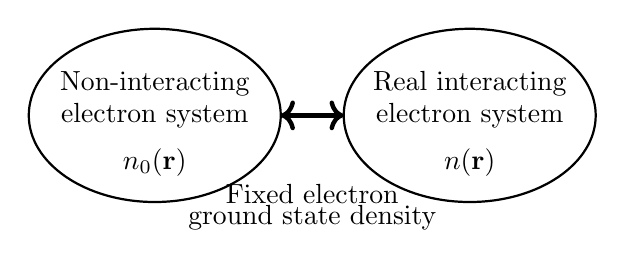
\begin{tikzpicture}
        \draw[thick] (-2,0) ellipse (1.6cm and 1.1cm);
        \draw[thick] (2,0) ellipse (1.6cm and 1.1cm);
        \draw[ultra thick,<->] (-0.4,0)--(0.4,0);
        \node[] at (-2,0.4) {Non-interacting};
        \node[] at (-2,0) {electron system};
        \node[] at (-2,-0.6) {$n_0(\vb{r})$};
        \node[] at (2,0.4) {Real interacting};
        \node[] at (2,0) {electron system};
        \node[] at (2,-0.6) {$n(\vb{r})$};
        \node[] at (0,-1) {Fixed electron};
        \node[] at (0,-1.3) {ground state density};
    \end{tikzpicture}
    \caption{Kohn-Sham ansatz}
    \label{fig:dft_ks_ansatz}
\end{figure}
This paper will in terms of \emph{Density Functinal Theory} (DFT) mainly focus on the self-consistent Kohn-Sham (KS) approach which was used in the computational part of the project. One can say that the self-consistent single-particle equations proposed by Hartree back in 1928 set the frame for the Kohn-Sham equations. \\ Back in 1964, Pierre Hohenberg and Walter Kohn took the first huge step in the development of modern DFT by proving that knowing the electron density in the ground state is enough for one to describe the whole system. In the winter of 1964, Kohn and Lu Jeu Sham then sat together and combined the Hohenberg-Kohn variational principle which in theory was exact for the ground-state together with the Hartree equations to form an, in principle, exact Hartree-like formulation, the Kohn-Sham equations.
\cite{KohnNobelLecture} \\
The Kohn-Sham approach is based on the assumption that one can find a ground state density for a fictitious system of non-interacting particles corresponding to the exact ground state density for the real interacting electron system as illustrated in figure \ref{fig:dft_ks_ansatz}. This non-interacting reference system is described by an effective potential and the usual kinetic term,
\begin{equation} 
\label{eq:reference_system_KS}
\hat{H}_R = - \dfrac{\hbar^2}{2m} \nabla^2 + v_R \qty(\vb{r})
\end{equation}
The difficult part in the Kohn-Sham ansatz is then to find such an effective potential for a given system which satisfies that the ground-state density can be written as a probability distribution over the single particle eigenfunctions; mathematically speaking,
\begin{equation}
\hat{H}_R = \varepsilon_i \phi_i \qty(\vb{r}) \qquad \qquad \sum_{i=1}^N \abs{\phi_i \qty(\vb{r})}^2 = n_0 \qty(\vb{r})
\end{equation}
Walter Kohn and Lu Jeu Sham got the idea to rewrite the Hohenberg-Kohn energy functional into large knows terms and put the unknowns into a new term, the so-called \emph{exchange-correlation functional}, $E_{xc}[n]$,
\begin{equation}\label{eq:kohn_sham_ef}
\begin{split}
    E[n] &= T[n] + U_{ee} [n] + \int v_{ion} \qty(\vb{r}) n \qty(\vb{r}) \difd \vb{r} \\
    &=T_s\qty[n] + U_{ee} \qty[n] + \int v_{ion} \qty(\vb{r}) n \qty(\vb{r}) \mathrm{d}\vb{r} + E_{xc} \qty[n] \\
    &= \underbrace{T_s \qty[n]}_\text{Non-interacting} + \underbrace{\dfrac{1}{2} \int \int \dfrac{n\qty(\vb{r'}) n\qty(\vb{r})}{\qty|\vb{r}-\vb{r'}|} \mathrm{d}\vb{r'} \, \mathrm{d}\vb{r}}_\text{Hartree} + \int v_{ion} \qty(\vb{r}) n \qty(\vb{r}) \mathrm{d}\vb{r} + \underbrace{ E_{xc} \qty[n]}_\text{Exchange-Correlation}
\end{split}
\end{equation}
In \eqref{eq:kohn_sham_ef}, the interacting kinetic energy term is split up to a non-interactive term plus a correlation term which is put into $E_{xc}[n]$. This means that this this fictitious wave function constructed by the eigenfunctions is treated as a single Slater determinant even though the real wave function can not. If this can be done under the constraint that the electron density remains the same, one can in principle obtain the right ground state energy even though the individual terms in the expression might be off energy-wise. However, the exact ground state energy can only be evaluated if the right exchange-correlation functional is used. And unfortunately, it is non an easy tasks to construct these functionals. The $U_{ee}[n]$ term in \ref{eq:kohn_sham_ef} is split up into the term one may know from classical Hartree theory and an unknown exchange-correlation term put into $E_{xc}[n]$ as well. \\

By using Euler's equation and Lagrange multipliers to assure particle conservation on \eqref{eq:kohn_sham_ef} and \eqref{eq:reference_system_KS}, one can combine the two Euler-Lagrange equations to obtain the effective potential, $v_R \qty(\vb{r})$:
\begin{equation}\label{eq:CombiningEuler}
\begin{split} 
v_R \qty(\vb{r}) &= \int \dfrac{n \qty(\vb{r'})}{\abs{\vb{r}-\vb{r'}}} \difd\vb{r'} + v_{ion} \qty(\vb{r}) + \dfrac{\delta E_{xc} \qty[n]}{\delta n } \\
&= v_H \qty(\vb{r}) + v_{ion} \qty(\vb{r}) + v_{xc} \qty(\vb{r})
\end{split}
\end{equation}
With this effective potential, one can try to solve single-particle Schrödinger's equations for the reference system. This is known as the Kohn-Sham self-consistency problem and in this way, Kohn and Sham created a density functional based formulation of Hartree's  work.

\subsection{The Kohn-Sham self-consistency equations}
\begin{figure}[h!]
    \centering
    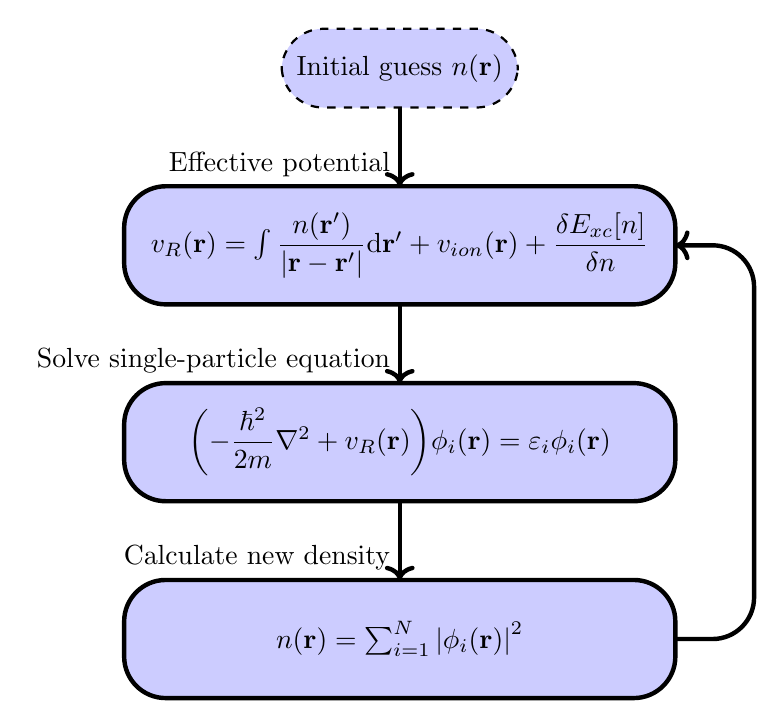
\begin{tikzpicture}
        \filldraw[fill=blue!20!white,dashed, thick, rounded corners=15pt] (-1.5,3) rectangle (1.5,4);
        \filldraw[fill=blue!20!white,ultra thick, rounded corners=15pt ] (-3.5,0.5) rectangle (3.5,2);
        \filldraw[fill=blue!20!white,ultra thick, rounded corners=15pt] (-3.5,-2) rectangle (3.5,-0.5);
        \filldraw[fill=blue!20!white,ultra thick, rounded corners=15pt] (-3.5,-4.5) rectangle (3.5,-3);
        \draw[ultra thick,->, rounded corners=15pt] (3.5,-3.75)--(4.5,-3.75)--(4.5,1.25)--(3.5,1.25);
        \draw[->, ultra thick] (0,3)--(0,2);
        \draw[->, ultra thick] (0,0.5)--(0,-0.5);
        \draw[->, ultra thick] (0,-2)--(0,-3);
        \node[] at (0,3.5) {Initial guess $n(\vb{r})$};
        \node[] at (0,1.25) {$v_R \qty(\vb{r}) = \int \dfrac{n \qty(\vb{r'})}{\abs{\vb{r}-\vb{r'}}} \difd\vb{r'} + v_{ion} \qty(\vb{r}) + \dfrac{\delta E_{xc} \qty[n]}{\delta n }$};
        
        \node[] at (0, -1.25) {$\qty(- \dfrac{\hbar^2}{2m} \nabla^2 + v_R \qty(\vb{r}))\phi_i\qty(\vb{r})=\varepsilon_i\phi_i\qty(\vb{r})$};
        \node[] at (0,-3.75) { $n\qty(\vb{r})= \sum_{i=1}^N \abs{\phi_i \qty(\vb{r})}^2$ };
        \node[anchor=south east] at (0,2) {Effective potential};
        \node[anchor=south east] at (0,-0.5) {Solve single-particle equation};
        \node[anchor=south east] at (0,-3) {Calculate new density};
    \end{tikzpicture}
    \caption{Hartree-like self-consistency problem}
    \label{fig:self_consistency_KS}
\end{figure}
This self-consistency problem looks a lot like Hartree's. The difference is in the inclusion of an exchange-correlation term. \\ 
As shown in figure \ref{fig:self_consistency_KS}, the procedure starts with a guess for the ground state density to which the effective potential can be constructed and Schrödinger's time-independent eigenvalue problem can be solved. These eigenfunctions then corresponds to a new density which is then put into the effective potential. The iterations continue until the ground state density is reached corresponding to the lowest energy. \\
In the Kohn-Sham approach, the ground state energy can be found to be given as \eqref{ground_state_energy}
\begin{equation}\label{ground_state_energy}
    E = \sum _j \varepsilon_j + E_{xc} \qty[n(\vb{r})]- \int v_{xc} (\vb{r}) n (\vb{r}) \dd v - \dfrac{1}{2} \int \dfrac{n(\vb{r}) n(\vb{r'})}{\abs{r-r'}}
\end{equation}

Having said that, the exchange-correlation functional, $E_{xc}[n]$, remains unknown and has to be approximated. Nowadays, there are huge databases with exchange-correlation functional and one may choose different functionals depending on what atomic property one is seeking to calculate. The choice of functional also depends on how accurate the calculation needs to be due to the time consumption being highly functional dependent. Jacob's ladder is often used in terms of DFT; the more accurate the simulation needs to be, the more expensive it is in terms of time/computation. \\
In this project, mainly a generalized gradient approximation (GGA) functional by the name PBE after Perdew,Burke and Ernzerhof has been used. The general stucture of a GGA functional is,
\begin{equation}
    E_{xc}[n]= \int n \qty(\vb{r}) \varepsilon_{xc} \comm{n\qty(\vb{r})}{ \nabla n \qty(\vb{r})} \dd \vb{r}
\end{equation}
where $\varepsilon_{xc}$ is the exchange-correlation hole. The GGA functional, PBE, was mainly chosen because of the relatively low computational costs and band structure preserving properties.

\subsection{Static screening, $\omega = 0$}
\paragraph{Thomas-Fermi model} (
\textbf{PROVE} that the induced potential from a plane-wave external potential must also be a plane-wave with the same wave vector.)\\
Relating the external and total potential:
\begin{equation}
\begin{split}
    U_{ext}(r) &= A_{ext}(q) \mathrm{e}^{iqr} + c.c \\
    U_{tot}(r) &= A_{tot}(q) \mathrm{e}^{iqr} + c.c
\end{split}
\end{equation}
where the induced electron density due to the external potential is, $n_{ind} = - \rho\qty(E_F) U_{tot}(r)$.

\paragraph{Remember the following FT:}
\begin{equation}
    \dfrac{1}{r}= \int  \dfrac{1}{q^2} \mathrm{e}^{i \vb{q}\cdot \vb{r}} d\vb{q}
\end{equation}
\paragraph{NB.} Potentials are exponentially screened in TF theory. In metals, $k_F^{-1} \approx a_0 \approx 0.5$Å. 

\subsection{Dynamical screening, $q =  0$}


\section{Week 4}\label{sec:week4}

\paragraph{Optical Regime} $q \to 0$, $\hbar \omega = \{1-3\}\mathrm{eV}$

\paragraph{Non-retarded regime} $(\omega \ll cq)$ and $(\omega \gg \nu_F q)$ 


$A(t) = \int_{\mathrm{conv}} B(t) C(t) dt \Rightarrow A(\omega) = B(\omega) C(\omega)$
or equivalently \\
$A(r) = \int_{\mathrm{conv}} B(r) C(r) dr \Rightarrow A(k) = B(k) C(k)$
\section{Week 5}

\begin{tikzpicture}
    % Axes
    \draw[->] (-5,0) -- (10,0) node[right] {$\omega$};
    \draw[->] (0,-5) -- (0,5) node[above] {$\epsilon$};
    
    % Ticks
        %y
        \draw (0,4.5) -- (-0.2,4.5) node[left] {\tiny{$\varepsilon_0 + 2t$}};
        \draw (0,2.5) -- (-0.2,2.5) node[left] {\tiny{$\varepsilon_0$}};
        \draw (0,0.5) -- (-0.2,0.5) node[left] {\tiny{$\varepsilon_0 - 2t$}};
        
        %x
        \draw (-pi,0)   -- (-pi,-0.2)    node[below] {\tiny{$-\frac{\pi}{a}$}};
        \draw (-pi/2,0) -- (-pi/2,-0.2)  node[below] {\tiny{$-\frac{\pi}{2a}$}};
        \draw (0,0)     -- (-0,-0.2)     node[below] {$0$};
        \draw (pi/2,0)  -- (pi/2,-0.2)   node[below] {\tiny{$\frac{\pi}{2a}$}};
        \draw (pi,0)    -- (pi,-0.2)     node[below] {\tiny{$\frac{\pi}{a}$}};
    
    % Legend
    \draw (-pi-0.2,1.5) -- (-pi+0.1,1.5) node[right] {\tiny{$\varepsilon(k)$ prob. 2.2}};
    \draw[dashed] (-pi-0.2,1) -- (-pi+0.1,1) node[right] {\tiny{$\varepsilon(k)$  prob. 2.3}};
    \draw (-pi-0.2,0.5) -- (-pi+0.1,0.5) node[right] {\tiny{$D(\varepsilon)$}};
    \filldraw[fill=black!5!white] (-pi-0.2,0.35) rectangle (-pi+0.1,0.65);
    
    % DOS
    %\filldraw[color=black,fill=black!5!white,smooth,samples=1000,variable=\y,domain=0.525:4.475] (0,0.5) -- (pi,0.5) plot ({(1/2)/(sqrt(1-(\y-2.5)*(\y-2.5)/4))},{\y}) --(pi,4.5) -- (0,4.5) -- (0,0.5);
    
    % Bands
    %\filldraw[color=black,fill=black!5!white,smooth,samples=100,domain=-4:4] (-4,0) -- plot (\x,{3*exp(-(\x-0.2)*(\x-0.2)/0.005)-3*exp(-(\x+0.2)*(\x+0.2)/0.005)}) -- (-4,0);
    \draw[color=black,smooth,samples=100,domain=1:4] plot (\x,{1-4/((\x)*(\x)))});
    %\draw[color=black,dashed,smooth,domain=(pi/2):pi]  plot (\x-pi,{2.5-2*cos(\x r)});
\end{tikzpicture}

\section{Week 6}
\textbf{Reading Material [GP]:}
\begin{itemize}
    \item 529-539 about band-to-band transitions
    \item 288-296 about excitons 
    \item 549-553 about the effect of excitons on the optical properties
\end{itemize}
\rule{\textwidth}{1pt}
\emph{Kristian's Appetiser:}
The first part concerns the description of optical absorption by band-to-band transitions. This is a single-particle picture which assumes that the electron in the conduction band and the hole left behind in the valence band, do not interact. This is an approximation which is, however, valid in many (important) situations, in particular for absorption above the band gap. Excitons are bound electron-hole pairs that form due to the attractive Coulomb interaction between the electron and the hole. They are mainly important in crystals where screening is weak, i.e. in insulators with low dielectric constants and/or in low dimensional structures such as 2D materials where the screening is weak due to geometrical constraints on the motion of the electrons. Excitons influence the optical properties, such as the absorption spectrum, by introducing discrete spectral lines below the band gap.They are mainly important when the exciton binding energy (the energy of the exciton relative to the band gap) is larger than the thermal energy $k_{B}T$ (25 meV at room temperature).
\rule{\textwidth}{1pt} \\
\paragraph{Dipole approximation} Where the wavelength of the incident radiation is much larger than the lattice parameter; in these situations, the photon wavevector $\vec{q}$ of the incident radiation is small compared to the range of values of $\vec{k}$ within the first Brillioun Zone (FBZ) and thus we neglect the $\vec{q}$-dependence and set $\vec{k}_j = \vec{k}_i$ corresponding to vertical/direct transitions.

In regards to the imaginary part of the dielectric function, this implies that
\begin{equation}
\begin{split}
    \varepsilon_2\qty(\omega) &= \dfrac{8\qty(\pi e)^2 }{\qty(m \omega)^2} \dfrac{1}{V} \sum_{cv} \sum_{\kkk} \abs{\mel{\psi_{c\kkk}}{\hat{\eee}\cdot \ppp}{\psi_{v\kkk}}}^2 \delta \qty(E_{c\kkk} - E_{v\kkk} - \hbar \omega) \\
    &= \dfrac{8\qty(\pi e)^2 }{\qty(m \omega)^2}  \sum_{cv} \int_{B.Z.} \dfrac{d\kkk}{\qty(2\pi)^3} \abs{\hat{\vec{e}} \cdot \mathrm{\mathbf{M}}_{cv}\qty(\kkk)}^2\delta \qty(E_{c\kkk} - E_{v\kkk} - \hbar \omega )
\end{split}
\end{equation}
where $\mathrm{\mathbf{M}}_{cv}\qty(\kkk)$ denotes the dipole matrix element $\mel{\psi_{c\kkk}}{\ppp}{\psi_{v\kkk}}$ and the sum runs over every couple of valence and conduction bands. 

Furthermore, the matrix elements $  \mel{\psi_{c\kkk}}{\mathrm{e}^{i \qqq \cdot \rrr}\hat{\eee}\cdot \ppp}{\psi_{v\kkk}}$ is typically denoted \textbf{the oscillator strength}.

\paragraph{DOS vs JDOS} \emph{The DOS is the number of states available with the same energy whereas the JDOS is the number of single particle transitions available for a given energy $E$.}

\textbf{NB.:} One can always choose a gauge such that the scalar potential vanishes $\Rightarrow \chi = \int_{-\infty}^t \phi\qty(r,t') dt'$. However, this is only valid for transverse waves.\\


\section{Week 8}
The retarded density-density response function can be used to obtain the longitudinal dielectric function of a material due to the relation between the induced potential and the induced electron density. Furthermore, it is useful when trying to identify \textit{neutral} excitations of the electron system. Such excitations include single-particle transition, plasmons and excitons. 

Conversely, charged excitations can be described by another correlation function, namely, the one-particle Green's function (GF). More precisely, charged excitations are excitations where the number of electrons in the electron system changes by $\pm 1$, e.g. photo-emission or STM.\footnote{Charged excitations do sometimes go under the name of addition/removal energies, anti-particle energies or one-electron energies.} 
The energies of charged excitations, $E_i \qty(N\pm1) - E_0\qty(N)$ are differences between exact many-body energy levels and thus completely well-defined. These types of excitations will from now on be denoted quasiparticles (QP).

\paragraph{The Retarded Green's function} is defined in real time and space as
\begin{equation}
    G\qty(x,x') = -i \theta\qty(t-t') \mel{N}{\{\fop{x},\fopd{x'}\}}{N}
\end{equation}
where $x = (r,t)$ and $\fop{x}=\expe{iHt}\fop{r} \expe{-iHt}$ is the annihilation operator in the Heisenberg picture.\footnote{In the following we assume that $\hat{H}$ is time-independent.}
Note that the two terms from the anti=
\end{document}
